% Este es el archivo consolidado de graficas\n
 \documentclass{article}
\usepackage[top=1cm,bottom=1cm,left=1cm,right=1cm]{geometry}
\usepackage{graphicx}

 \begin{document}
 
 \centerline{\textbf{\Large Preliminary data analysis of pilot run May 2nd 2019}}
 
\section{Participants and experimental task} 
The participants were 20 students at the Universidad del Rosario. The experiment was conducted in the Laboratory for Experimental Economy in sight isolated computers. Players were grouped into 10 dyads but they did not know who was paired with whom. They were instructed not to talk to each other.  

\

The task consisted in 20 rounds of training and 25 rounds of game. During each round, players were required to classify the images of 5 dogs. During the rounds of \emph{training}, each player was required to classify 5 dogs from two different categories and each player in the dyad observed different categories from their partner. At the end of the round, participants were shown a feedback screen with their correct and incorrect responses, as well as the score history over the last 20 rounds. During the rounds of \emph{game}, each player was required to classify 5 dogs from four different categories (the two categories they were trained into, and the two categories their partner was trained into). At the end of the round, participants were shown a feedback screen with their correct and incorrect responses, as well as the score history over the last 20 rounds. 

\

Each player received a monetary reward for their performance during the task. They received around 0.3 dollars for showing up and finishing the task to the end, and up to around 3 dollars for their performance on two randomly chosen rounds during the rounds of game. The average time for participants to complete the task was 54 minutes.

\section{Training rounds}
The first question we want to answer is the extent to which players became proficient in discriminating dogs in the two categories that were presented to them during the rounds of training. If players did not acquire a good degree of proficiency, they would not be reliable sources of information for the rounds of game. Figs.~1 and 2 show that players did not substantially improve their classification skills (no error regions, sorry!) and Fig.~3 shows that the situation was similar for all four categories (no error bars, sorry!).

\ 

\begin{tabular}{cc}
Average Score & Average Accumulated Score \cr 
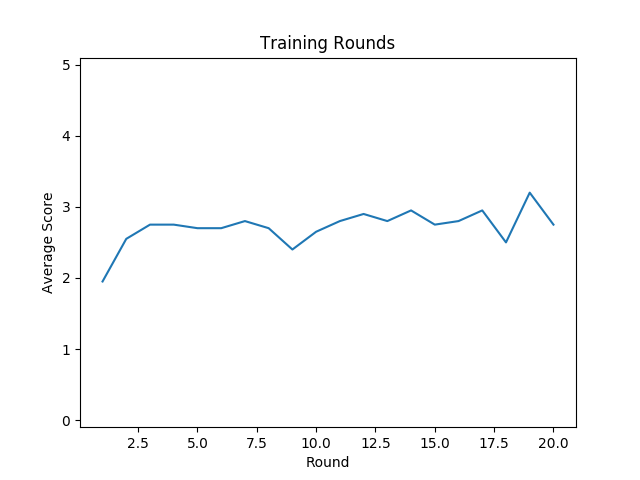
\includegraphics[scale=0.45]{Graficas/Stage1/score.png} &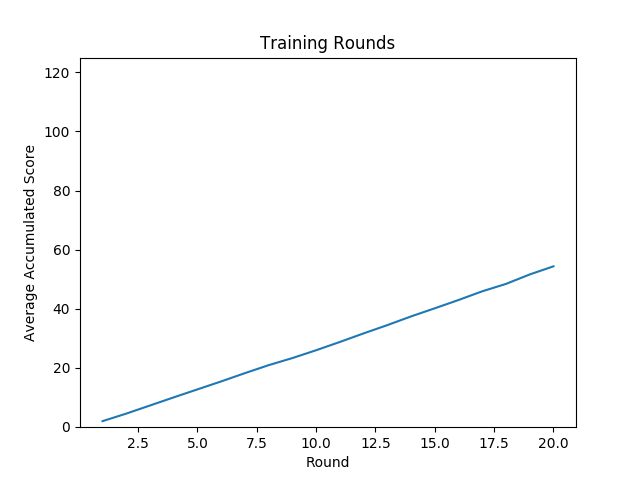
\includegraphics[scale=0.45]{Graficas/Stage1/ac_score.png} \cr 
Fig. 1: Score per round, averaged over 20 participants. & Fig. 2: Accumulated score per round, averaged over 20 participants.\cr
\multicolumn{2}{c}{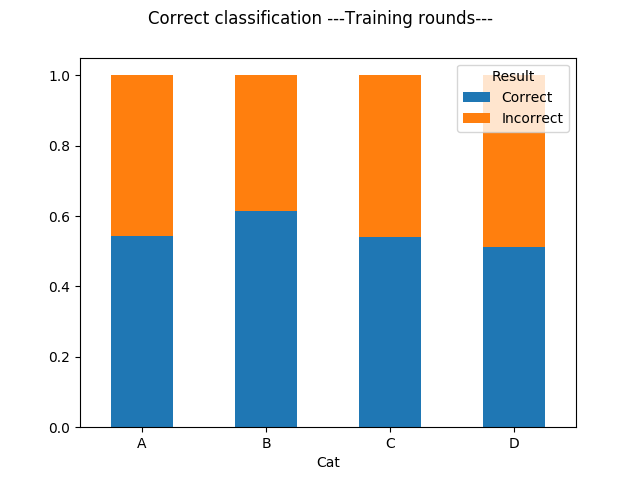
\includegraphics[scale=0.45]{Graficas/correctClassTraining.png}}\cr
\multicolumn{2}{c}{Fig. 3: Classification accuracy per category during rounds of training.}
\end{tabular}

\newpage

\section{Game Rounds}
The second question is the extent to which players were able to classify dogs during rounds of game. Figs.~4 and 5 shows that, not surprisingly, the situation is just as bad as in the rounds of training. Fig.~6 shows that the discrimination accuracy is only slightly better in the case of the two categories to which the participant was trained (``trained categories'') during the rounds of training. 

\ 

\begin{tabular}{cc}
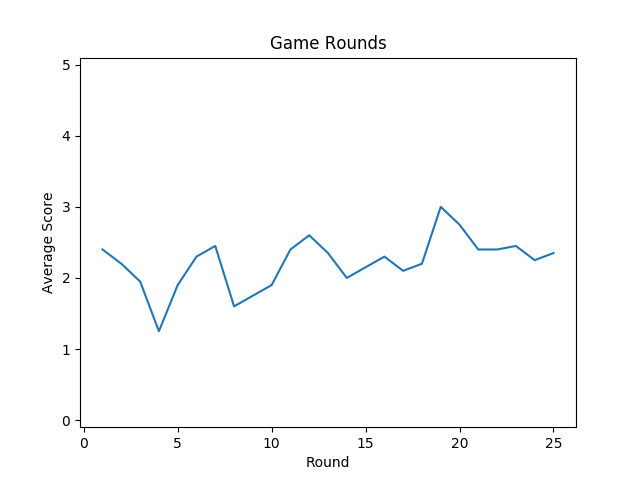
\includegraphics[scale=0.4]{Graficas/Stage2/score.png} &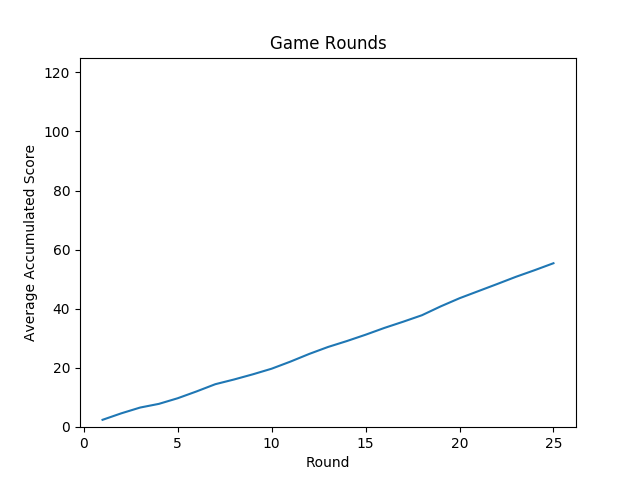
\includegraphics[scale=0.4]{Graficas/Stage2/ac_score.png} \cr 
Fig. 4: Score per round, averaged over 20 participants. & Fig. 5: Accumulated score per round, averaged over 20 participants.\cr
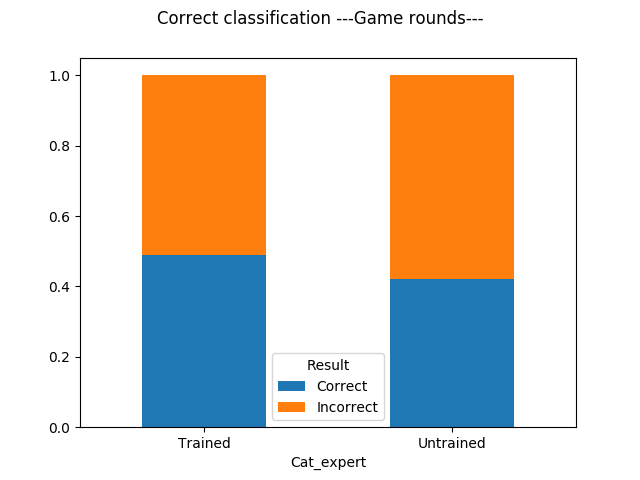
\includegraphics[scale=0.4]{Graficas/correctClassGame.png} & 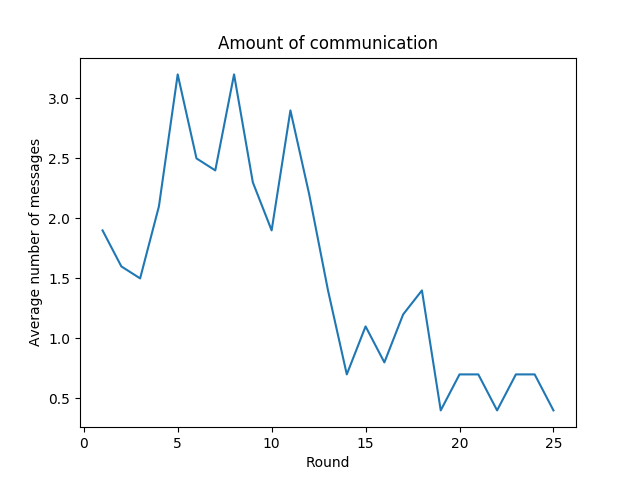
\includegraphics[scale=0.4]{Graficas/amount_comm.png} \cr
Fig. 6: Classification accuracy for ``trained categories''\\ and ``untrained categories''  during rounds of game. & Fig. 7: Amount of messages per round, averaged over 20 participants.
\end{tabular}

\

The third question is the extent to which players communicate with each other. Fig.~7 shows that players sent an average of 2 messages during the initial rounds. The average rises above three messages per round, perhaps because participants found the task very hard and where procuring assistance from their partner. But from there on, the number of messages per round drops dramatically, no doubt because their partner was not doing any better at the classification task.

\

The fourth question is whether the scheme of communication was clear to the players. Figs.~8 and 9 show the relative frequency of each response given to the categorization task after they received an affirmative/negative answer from a query posed to their partner. Fig.~8 shows that players trusted their partner's classification when the response was affirmative. Thus, for example, they tended to classify a dog as an A when the answer to their query ``This dog is an A?'' was affirmative. We were expecting that they would be able to infer that a negative response pointed in the direction of the other category (that is, choose C when partner says that the dog is not A). Fig.~9 shows that this was not the case. Classifications are all over the place when players obtained a negative response from their partner to their query.

\

\begin{tabular}{cc}
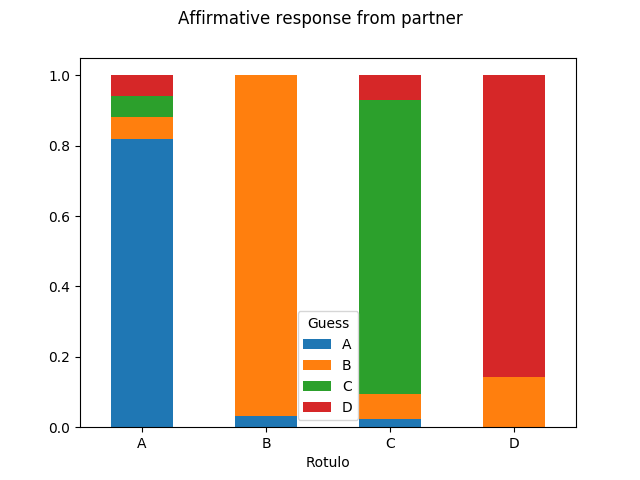
\includegraphics[scale=0.4]{Graficas/affResp.png} & 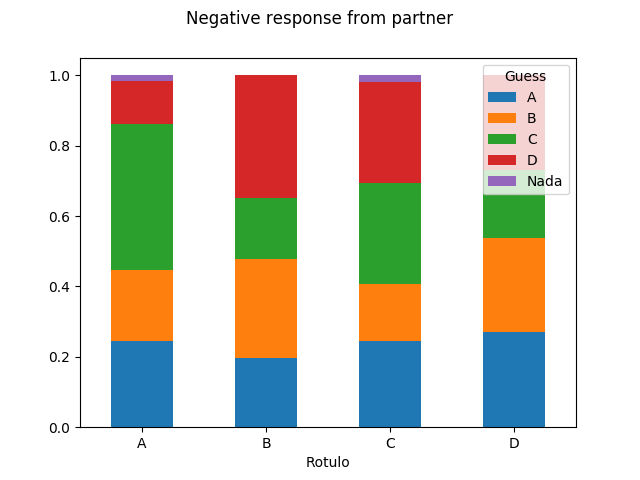
\includegraphics[scale=0.4]{Graficas/negResp.png} \cr
\multicolumn{1}{p{0.4\textwidth}}{Fig. 8: Relative frequencies of classifications after a query per category, when the response to the query was affirmative.} & \multicolumn{1}{p{0.4\textwidth}}{Fig. 9: Relative frequencies of classifications after a query per category, when the response to the query was negative.}\cr
\end{tabular}


 \end{document}
